\documentclass{article}[11pt]
\usepackage{fullpage,graphicx, setspace, latexsym, cite,amsmath,amssymb,xcolor,subfigure}
%\usepackage{epstopdf}
%\DeclareGraphicsExtensions{.pdf,.eps,.png,.jpg,.mps} 
\usepackage{amssymb} %maths
\usepackage{amsmath} %maths
\usepackage{amsthm, comment}
\usepackage[round,comma,sort,numbers, compress]{natbib}

% \bibliographystyle{plain}
\bibliographystyle{plos2015}

\newtheorem{theorem}{Theorem}
\newtheorem{prop}{Proposition}
\newtheorem{corollary}{Corollary}
\newtheorem{lemma}{Lemma}
\newtheorem{defn}{Definition}
\newtheorem{ex}{Example}
\usepackage{float}

\newcommand*{\underuparrow}[1]{\underset{\uparrow}{#1}}
\usepackage{graphicx}
\usepackage{xcolor}
\usepackage[dvipsnames]{xcolor}
\usepackage{algorithmicx}
\usepackage{algorithm} %http://ctan.org/pkg/algorithms
\usepackage{algpseudocode} %http://ctan.org/pkg/algorithmicx
\usepackage{enumitem}
\usepackage{simplemargins}
\usepackage{hyperref}
\hypersetup{
     colorlinks=true,
     linkcolor=blue,
     filecolor=red,
     citecolor = red,      
     urlcolor=cyan,
}

\usepackage{mdframed}
\definecolor{lgray}{rgb}{0.92,0.92,0.92}
\definecolor{lsalmon}{rgb}{0.9921568627450981,0.9411764705882353, 0.9254901960784314}

\renewcommand{\bibnumfmt}[1]{#1.}
\setlist{noitemsep} % or \setlist{noitemsep} to leave space around whole list
\setallmargins{1in}
\linespread{1.1}

\newcommand{\brows}[1]{%
  \begin{bmatrix}
  \begin{array}{@{\protect\rotvert\;}c@{\;\protect\rotvert}}
  #1
  \end{array}
  \end{bmatrix}
}
\newcommand{\rotvert}{\rotatebox[origin=c]{90}{$\vert$}}
\newcommand{\rowsvdots}{\multicolumn{1}{@{}c@{}}{\vdots}}


\def\R{\mathbb{R}}
\def\Eps{\mathcal{E}}
\def\E{\mathbb{E}}
\def\V{\mathbb{V}}
\def\F{\mathcal{F}}
\def\G{\mathcal{G}}
\def\H{\mathcal{H}}
\def\S{\mathcal{S}}
\def\D{\mathcal{D}}
\def\P{\mathbb{P}}
\def\1{\mathbf{1}}
\def\n{\nappa}
\def\h{\mathbf{w}}
\def\v{\mathbf{v}}
\def\x{\mathbf{x}}
\def\X{\mathcal{X}}
\def\Y{\mathcal{Y}}
\def\eps{\epsilon}
\def\y{\mathbf{y}}
\def\e{\mathbf{e}}
\newcommand{\norm}[1]{\left|\left|#1\right|\right|}
\DeclareMathOperator*{\argmin}{arg\,min}
\DeclareMathOperator*{\argmax}{arg\,max}
\newcommand{\lecture}[4]{
   \pagestyle{myheadings}
   \thispagestyle{plain}
   \newpage
   % \setcounter{lecnum}{#1}
   \setcounter{page}{1}
   \setlength{\headsep}{10mm}
   \noindent
   \begin{center}
   \framebox{
      \vbox{\vspace{2mm}
    \hbox to 6.28in { {\bf CHEME 5820: Machine Learning for Engineers
   \hfill Spring 2025} }
       \vspace{4mm}
       \hbox to 6.28in { {\Large \hfill Lecture #1: #2  \hfill} }
       \vspace{2mm}
       \hbox to 6.28in { {\it Lecturer: #3 \hfill #4} }
      \vspace{2mm}}
   }
   \end{center}
   \markboth{Lecture #1: #2}{Lecture #1: #2}

   \noindent{\bf Disclaimer}: {\it These notes have not been subjected to the
   usual scrutiny reserved for formal publications. }
   \vspace*{4mm}
}

\begin{document}
\lecture{5b}{Flux Balance Analysis (FBA)}{Jeffrey Varner}{}

\begin{mdframed}[backgroundcolor=lgray]
    In this lecture, we will discuss the following topics:
    \begin{itemize}[leftmargin=16pt]
      \item{\href{sec:FBA}{Flux Balance Analysis (FBA)} is a mathematical approach for analyzing the steady-state flow of carbon and energy through a metabolic network operating in some abstract volume, e.g., a cell, a test tube, or a logical compartment. The flow of material through the reaction network is called the metabolic flux. We estimate metabolic flux using \href{https://en.wikipedia.org/wiki/Linear_programming}{linear programming} (not the only approach, but the one that we will start with).} 
      \item{\href{sec:FBA}{Metabolic flux}, the rate of molecular flow in reaction pathways, is crucial for understanding cellular operations. It reveals how cells manage energy production, utilize nutrients, and respond to environmental changes, making it vital for studying diseases, drug development, and optimizing bioprocesses.}
      \item{\href{sec:linear-programming}{Linear programming} is an optimization technique used to find the best outcome in a mathematical model whose requirements are represented by linear relationships, e.g., the maximization (minimization) of a linear objective function subject to linear equality, inequality, and bounds constraints.}
    \end{itemize}
 \end{mdframed}

\section{Introduction}
In the previous lecture, we discussed the stoichiometric matrix $\mathbf{S}$, which is a mathematical representation of a metabolic network. 
The stoichiometric matrix encodes the relationships between reactants and products in the network, where rows correspond to different metabolites, contained in the set $\mathcal{M}$, and columns correspond to reactions, contained in the set $\mathcal{R}$. 
Thus, the stoichiometric matrix is a $\mathbf{S}\in\mathbb{R}^{|\mathcal{M}|\times|\mathcal{R}|}$ matrix holding the stochiometric coefficients $\sigma_{ij}\in\mathbf{S}$ for $i=1,2,\dots,|\mathcal{M}|$ and $j=1,2,\dots,|\mathcal{R}|$. 
In this lecture, we will discuss how we can use the stoichiometric matrix to analyze the metabolic network and predict the fluxes through the network using a technique called Flux Balance Analysis (FBA).
In particular, we will explore the ideas in the paper by Orth et al \cite{Orth:2010aa}.

\section{Material Balance Equations}
Before we dive into FBA, let's first consider the material balance equations for a metabolic network. 
These form the constraints that we will use in FBA.
Each metabolite, enzyme, genem, mRNA species in the metabolic network is subject to a material balance equation, which describes the rate of change of the concentration of the metabolite (enzyme, etc) in the system.
Material balance equations are a fundamental concept in chemical engineering that can bbe applied to many different types of systems, including metabolic networks.
Material balances consist for four types of terms: accumulation, generation, transport in and out of the system.

Imagine we have an \texttt{abstract biophase}, which is a well-mixed compartment where our metabolic reactions are occuring.
This biophase can be a single cell, a compartment within a single cell, such as the cytoplasm or mitochondria, a cell-free system or a even collection of cells in 
a bioreactor. Let the volume of the biophase be $V$ (depending on the context, $V$ could be the volume of a single cell, the volume of the cytoplasm, cell number, cell mass, thus it will units specific to the case).
Then, we can write balances around each chemical species $i\in\mathcal{M}$ in the system as (Defn. \ref{defn-material-balance}):

\begin{mdframed}
\begin{defn}[Material Balance Equation]\label{defn-material-balance}
A material balance equation for species $i$ in a system with volume $V$ has four terms:
\begin{equation}\label{eqn-material-balance-words}
\text{Accumulation} = \text{Generation} + \text{Transport In} - \text{Transport Out}
\end{equation}
The \texttt{accumulation} term is the rate of change of species $i$ in the system, 
\texttt{generation} is the rate of production (consumption) of species $i$ by chemical reactions in the system,
the \texttt{transport} terms describe the rate of phyisical transport (convection or passive diffusion) of species $i$ into (from) the system.
\end{defn}
\end{mdframed}
Material balance equations can be written in terms of species concentration, the number of moles, or the species' mass.
The choice of units depends on the context of the problem, and the type of data available. 
However, we'll consider species mole balances and species concentration balances (as these are the most common types of material balances used in flux balance analysis).

\subsubsection*{Dynamic Species Mole Balances}
Suppose we have a system with volume $V$ in which we have a set of chemical species $\mathcal{M}$, a set of streams $\mathcal{S}$, and a set of chemical reactions $\mathcal{R}$.
Using the four tems in Defn. \ref{defn-material-balance}, we can write the dynamic species mole balance for species $i$ in the system.
Let $n_{i}$ denote the number of moles of chemical component $i\in\mathcal{M}$ (units: mol).
Further, each stream $s\in\mathcal{S}$ (flowing into or from) our volume has a direction parameter $d_{s}\in\left[-1,1\right]$. 
If stream $s$ enters the system $d_{s} = +1$, however is stream $s$ exits the system then $d_{s} = -1$.

\begin{mdframed}
\begin{defn}[Dynamic species mole balance]\label{defn-dynamic-species-mole-balance}
The number of moles of chemical component $n_{i}$ (unit: mol) in the system as a function of time is described by the 
open species mass balance equation:
\begin{equation}\label{eqn-species-mol-balance}
\sum_{s\in\mathcal{S}}d_{s}\dot{n}_{i,} + \dot{n}_{G,i} = \frac{dn_{i}}{dt}
\qquad\forall{i}\in\mathcal{M}
\end{equation}
where $\dot{n}_{i,s}$ denotes the mole flow rate of component $i$ in stream $s$ (units: mol $i$/time),
$\dot{n}_{G,i}$ denote the rate of generation of component $i$ in the system 
(units: mol-$i$/time), and $dn_{i}/dt$ denotes the rate of accumlation of the number of moles of component $i$ in the system (units: mol-$i$/time). 
Generation terms describe the impact of chemical reactions.
The species generation rate $\dot{n}_{G,i}$ can be written in terms of the open extent of reaction:
\begin{equation}\label{eqn-open-extent-species}
\dot{n}_{G,i} = \sum_{r\in\mathcal{R}}\sigma_{ir}\dot{\epsilon}_{r}
\end{equation}
where $\sigma_{ir}$ denotes the stoichiometric coefficient of species $i$ in reaction $r$, and $\dot{\epsilon}_{r}$ denotes the open extend of reaction $r$ (units: mol/time).
Putting these ideas together, we can rewrite the dynamic species mole balance as:
\begin{equation}\label{eqn-dynamic-smb-with-extent}
\sum_{s\in\mathcal{S}}d_{s}\dot{n}_{i,s} + \sum_{r\in\mathcal{R}}\sigma_{ir}\dot{\epsilon}_{r} = \frac{dn_{i}}{dt}\qquad\forall{i\in\mathcal{M}}
\end{equation}
\end{defn}
\end{mdframed}

\subsubsection*{Dynamic Species Concentration Balances}
When describing systems with chemical reactions we write reaction rate expressions in terms of 
concentration, e.g., mole per unit volume basis.
In these cases, we need a new balance equation, the concentration balance. 
Let $n_{i}$ denote the number of moles of chemical component $i$ in the system (units: mol). 
Using the four terms in Defn. \ref{defn-material-balance}, we can write the dynamic species concentration balance for species $i$ in the system.

\begin{mdframed}
\begin{defn}[Dynamic Species Concentration Balance]\label{defn-dynamic-species-concentration-balance}
Starting with the species mole balances (Defn \ref{defn-dynamic-species-mole-balance}), we can re-write the number of moles of species $i$ as $n_{i} = C_{i}V$ for ${i}\in\mathcal{M}$
where $C_{i}$ denotes the concentration of species $i$ (units: mole per volume), and $V$ (units: volume) denotes the volume of the system. 
Thus, we can re-write the species mole balance in concentration units as:
\begin{equation}\label{eqn:concentration-balance}
\sum_{s\in\mathcal{S}}d_{s}C_{i,s}\dot{V}_{s} + \dot{C}_{G,i}V = \frac{d}{dt}\left(C_{i}V\right)\qquad\forall{i}\in\mathcal{M}
\end{equation}
where $\dot{V}_{s}$ denotes the volumetric flow rate for stream $s$ (units: volume/time), 
$C_{i,s}$ denotes the concentration of component $i$ in stream $s$ (units: concentration), 
and $\dot{C}_{G,i}$ denotes the rate of generation of component $i$ by chemical reaction (units: concentration/time).
The generation terms for species $i$ in the concentration balance equation can be written as:
\begin{equation}\label{eqn:concentration-gen-terms}
\dot{C}_{G,i}V = \sum_{j\in\mathcal{R}}\sigma_{ij}\hat{v}_{j}V\qquad\forall{i}\in\mathcal{M}
\end{equation}
where $\sigma_{ij}$ denotes the stoichiometric coefficient of species $i$ in reaction $j$ (units: dimensionless), 
and $\hat{v}_{j}$ denotes the rate of the jth chemical reaction per unit volume (units: concentration/volume-time), 
and $V$ denotes the volume of the system (units: volume).
Putting these ideas together, we can rewrite the dynamic species concentration balances (in the system) as:
\begin{equation}\label{eqn:concentration-balance-with-extent}
\sum_{s\in\mathcal{S}}d_{s}C_{i,s}\dot{V}_{s} + \sum_{j\in\mathcal{R}}\sigma_{ij}\hat{v}_{j}V = \frac{d}{dt}\left(C_{i}V\right)\qquad\forall{i\in\mathcal{M}}
\end{equation}
\end{defn}
\end{mdframed}

\section{Flux balance Analysis}\label{sec:FBA}
Metabolic fluxes are the rates of the reactions in a metabolic network, which are the unknowns we want to estimate from various types of experimental data.
You can think of metabolic fluxes as the flow of metabolites through the metabolic network, which is analogous to water flow through a pipe.
Thus, estimating the metabolic fluxes is important for understanding the structure and operation of a metabolic network as a function of the environment.
Metabolic fluxes can be estimated using various mathematical methods, such as metabolic flux analysis (MFA) and flux balance analysis (FBA).
These two methods are based on different assumptions about the network, and they have different strengths and weaknesses.
We will focus on FBA, but for those interested in MFA, we recommend the review of Antoniewicz \cite{ANTONIEWICZ20212}.

\subsection{Linear Programming}\label{sec:linear-programming}
Flux balance analysis (FBA) is arguably the most widely used approach to estimate steady-state metabolic fluxes \cite{Orth:2010aa}. 
FBA is based on the assumption that the system is at a steady state, which means that the concentrations of the metabolites in the system are not changing with time.
This assumption allows us to estimate the fluxes through the network using linear programming.
While we'll introduce linear programming in the context of metabolic network analysis, 
it is a general tool that can be used to estimate flows through many different types of networks and graphs, e.g., social graphs, communication networks, or other types of problems that can be represented as a network of graphs.

\begin{figure}
  \centering
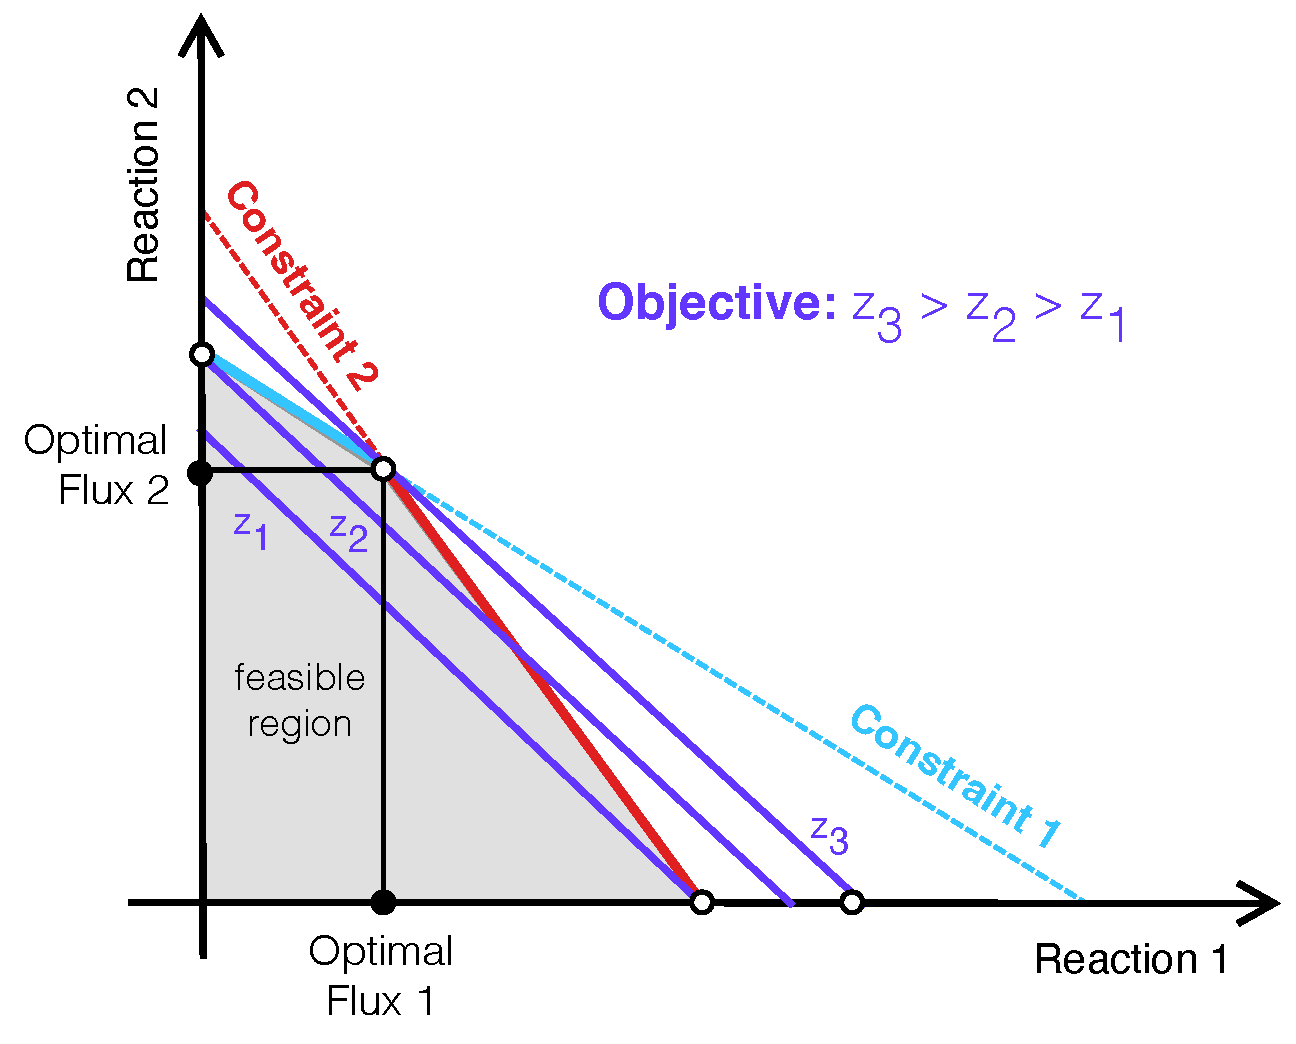
\includegraphics[width=0.64\textwidth]{./figs/Fig-LinearProgramming-Schematic.pdf}
\caption{Schematic of a two dimensional linear programming problem (maximization).
The optimal solution lies at the intersection between constraints (which define a feasible region) and the objective hyperplane with has the largest objective value.
In this case, the optimal solution is at the point $(x_{1}^{\star},x_{2}^{\star})$, which is where the objective function is maximized $z_{3}$.
}\label{fig:LinearProgramming-Schematic}
\end{figure}

Linear programming is an optimization technique used to find the best outcome in a mathematical model whose requirements are represented by linear relationships.
Linear programming maximizes (or minimizes) a linear objective function subject to linear equality, inequality, and bounds constraints.
The objective function is a linear combination of the decision variables, the unknowns we are trying to estimate.
The constraints are linear equations or inequalities describing the decision variables' relationships.

The solution to the linear program is the set of decision variables that maximize (or minimize) the objective function subject to the constraints (Fig. \ref{fig:LinearProgramming-Schematic}).
The constraints are linear equations or inequalities that describe the relationships between the decision variables.
The constraints form a feasible region in the space of the decision variables, and the optimal solution is the point in the feasible region that maximizes (or minimizes) the objective function.
The objective function is a linear combination of the decision variables, which are the unknowns we are trying to estimate, thus it is a hyperplane in the space of the decision variables.
The intersection objective function and the feasible region are potential solution points, where the optimal solution is the point that maximizes (or minimizes) the objective function.
We will not dig into the theory of linear programming, but we will use it to estimate the metabolic fluxes in a metabolic network using FBA.
For those interested in learning more about linear programming, we recommend \href{https://people.orie.cornell.edu/dpw/orie6300/}{the ORIE 6300 course notes by Prof. David Williamson}.

Let $\mathcal{O}(\mathbf{x})$ denote a linear function of the non-negative decision variables $\mathbf{x}\in\mathbb{R}^{n}$
whose values are constrained by a system of linear algebra equations and bounded. 
Then, the optimal decision $\mathbf{x}^{\star}\in\mathbb{R}^{n}$ is the solution of the linear program (written in standard form):
\begin{align*}
\max_{\mathbf{x}} &\quad \mathcal{O}(\mathbf{x}) = \sum_{i=1}^{n} c_{i}{x}_{i}\\
\text{subject to}&\quad\mathbf{A}\mathbf{x} \leq\mathbf{b}\\
\text{and} &\quad x_{i}\geq{0}\quad{i=1,2,\dots,n}
\end{align*}
where $c_{i}\in\mathbb{R}$ are constant coefficients in the objective function, $\mathbf{A}\in\mathbb{R}^{m\times{n}}$ 
is an $m\times{n}$ constraint matrix and $\mathbf{b}\in\mathbb{R}^{m}$ is an $m\times{1}$ right-hand side vector. 
Any linear program can be converted into this standard form.  

\subsection{FBA problem formulation}
FBA aims to estimate the intracellular reaction rates (fluxes) using whatever experimental data is available.
The more available data, the more constraints we can put on the system, and the more accurate our flux estimates will be.
However, one of the powerful aspects of FBA is that it can be used to estimate the metabolic fluxes even for a system in which we have very little data.
Suppose we have a system, with a species set $\mathcal{M}$, stream set $\mathcal{S}$ and a reaction set $\mathcal{R}$. 
Further, suppose that the system (or at least part of it) is at or near a steady state. 
The optimal reaction rates can be esimated using the following linear program (Defn. \ref{defn-fba-concentration}).

\begin{mdframed}
\begin{defn}[Flux Balance Analysis (FBA)]\label{defn-fba-concentration}
The flux balance analysis problem, whose solution provides estimates for the values of the unknown fluxes is the linear program: 
\begin{eqnarray*}
\text{minimize/maximize}~& & \sum_{i\in\mathcal{R}}c_{i}\hat{v}_{i}\\
\text{subject to} & & \sum_{s\in\mathcal{S}}\nu_{s}C_{s,i}\dot{V}_{s} + \sum_{j\in\mathcal{R}}\sigma_{ij}\hat{v}_{j}V = \frac{d}{dt}\left(C_{i}V\right)\qquad\forall{i\in\mathcal{M}}\\
\text{subject to} & & \mathcal{L}_{j}\leq\hat{v}_{j}\leq\mathcal{U}_{j}\qquad\forall{j\in\mathcal{R}}
\end{eqnarray*}
The $\sigma_{ij}\mathbf{S}$ are the elements of the  stoichiometric matrix $\mathbf{S}\in\R^{|\mathcal{M}|\times|\mathcal{R}|}$, 
the terms $c_{i}$ denote the objective coefficients, 
$\mathbf{v}$ denotes the unknown flux vector (the unknown that we are trying to estimate), and 
$\mathcal{L}$ ($\mathcal{U}$) denote the permissible lower (upper) bounds on the unknown fluxes. 
The first set of constraints are material constraints, 
while the second imparts thermodynamic and kinetic information into the calculation. 
Finally, there are potentially other types of constraints (both linear and nonlinear) not shown 
that may be necessary for specific applications encountered in practice.
\end{defn}
\end{mdframed}




\bibliography{References-W5.bib}

\end{document}